%%=====================================================================================
%%
%%       Filename:  lang-eng.tex
%%
%%    Description:  formal notes for lang-eng
%%
%%        Version:  1.0
%%        Created:  14/10/19
%%       Revision:  none
%%
%%         Author:  Josh Felmeden (), nk18044@bristol.ac.uk
%%   Organization:  
%%      Copyright:  Copyright (c) 2019, Josh Felmeden
%%
%%          Notes:  
%%
%%=====================================================================================

% Preamble {{{
\documentclass[11pt,a4paper,titlepage,dvipsnames,cmyk]{scrartcl}
\usepackage[english]{babel}
\typearea{12}
% }}}

% Set indentation and line skip for paragraph {{{
\setlength{\parindent}{0em}
\setlength{\parskip}{1em}
\usepackage[margin=2cm]{geometry}
\addtolength{\textheight}{-1in}
\setlength{\headsep}{.5in}
% }}}

\usepackage{hhline} 
\usepackage{mathtools} 
\usepackage[T1]{fontenc}

% Headers setup {{{
\usepackage{fancyhdr}
\pagestyle{fancy}
\lhead{Language Engineering - A nice set of notes}
\rhead{Josh Felmeden}
\usepackage{hyperref} 
% }}}

% Listings {{{
\usepackage[]{listings,xcolor} 
\lstset
{
    breaklines=true,
    tabsize=3,
    showstringspaces=false
}

\definecolor{lstgrey}{rgb}{0.05,0.05,0.05}
\usepackage{listings}
\makeatletter
\lstset{language=[Visual]Basic,
    backgroundcolor=\color{lstgrey},
    frame=single,
    xleftmargin=0.7cm,
    frame=tlbr, framesep=0.2cm, framerule=0pt,
    basicstyle=\lst@ifdisplaystyle\color{white}\footnotesize\ttfamily\else\color{black}\footnotesize\ttfamily\fi,
    captionpos=b,
    tabsize=2,
    keywordstyle=\color{Magenta}\bfseries,
    identifierstyle=\color{Cyan},
    stringstyle=\color{Yellow},
    commentstyle=\color{Gray}\itshape
}
\makeatother
\renewcommand{\familydefault}{\sfdefault}
% }}}


% Other packages {{{
\usepackage{tikz}
\usepackage{needspace}
\usepackage{tcolorbox}
\usepackage{soul}
\usepackage{babel,dejavu,helvet} 
\usepackage{amsmath,amsfonts} 
\usepackage{booktabs} 
\usepackage{tcolorbox} 
\usepackage[symbol]{footmisc} 
\renewcommand{\thefootnote}{\fnsymbol{footnote}}
\renewcommand{\familydefault}{\sfdefault}
\newcommand\pfun{\hookrightarrow}
% }}}

% Title {{{
\title{Language Engineering - A nice set of notes}
\author{Josh Felmeden}
% }}}

\begin{document}

\maketitle
\tableofcontents

\newpage

\section{Introduction to Semantics}%
\label{sec:intro-semantics}

Semantics are really complex and they actually exist in the real world as
problems that can arise when the semantics are unclear. In the example of
the Derek Bentley case, Bentley tells Chris (who is holding a gun, and a
policeman standing in front of him to `let him have it!'. Here, it
appears that he could be talking about the gun, or to kill him. The same
kind of thing can happen in computing when we are unsure of the references
of certain objects. 

Here are some examples learned from natural languages:
\begin{itemize}
    \item Syntactic complexity
        \begin{itemize}
            \item Jack built the house the malt the rat the cat killed ate
                lay in
        \end{itemize}
    \item Syntactic ambiguity
        \begin{itemize}
            \item Let him have it, Chris!
        \end{itemize}
        \item Semantic Complexity
            \begin{itemize}
                \item It depends on what the meaning of the word `is' is!
            \end{itemize}
        \item Semantic ambiguity
            \begin{itemize}
                \item I haven't slept for ten days
            \end{itemize}
            \item Semantic undefinedness
            \begin{itemize}
                \item Colourless green ideas sleep furiously
            \end{itemize}
            \item Interaction of syntax and semantics
                \begin{itemize}
                    \item Time flies like an arrow, fruit flies like a
                        banana.
                \end{itemize}
\end{itemize}

We can apply these things to computing terms, too.
\begin{itemize}
    \item Syntactic complexity
            \begin{lstlisting}
x-=y = (x=x+y) - y      //switches variables x and y
            \end{lstlisting}
    \item Syntactic ambiguity
\begin{lstlisting}
if (...) if (...) ..; else ..       //dangling else
\end{lstlisting}
        \item Semantic Complexity
\begin{lstlisting}
y = x++ + x++       //sequence points
\end{lstlisting}
        \item Semantic ambiguity
\begin{lstlisting}
(x%2=1) ? "odd" : "even"        //unspecified in C89 if x<0
\end{lstlisting}
            \item Semantic undefinedness
\begin{lstlisting}
while(x/x)      //division error or infinite loop
\end{lstlisting}
            \item Interaction of syntax and semantics
\begin{lstlisting}
A * B       //lever hack
\end{lstlisting}

\end{itemize}

To put this another way:
\begin{itemize}
    \item \textbf{Syntax}: concerned with the form of expressions and
        whether or not the program actually \textit{compiles}
    \item \textbf{Semantics}: concerned with the meaning of expressions
        and what the program does when it \textit{runs}
    \item \textbf{Pragmatics}: concerned with issues like design patterns,
        program style, industry standards, etc.
\end{itemize}

% 21/10/19
\section{Structural Operational Semantics}%
\label{sec:struct-op-semantics}
We're going to look at doing some compilation (of the \textit{while})
language.

\subsection{Termination and looping}%
\label{sub:term-loop}

The execution of the statement $S$ in state $\sigma$ terminates iff there
exists a finite derivation sequence from $\langle S, \sigma \rangle$. The
derivation sequence looks like:
\begin{align*}
    \langle S, \theta\rangle \Rightarrow \gamma_1 \Rightarrow \dots
    \Rightarrow \gamma_n \text{ where } \gamma_n \text{ is terminal }
    \sigma' \text{ or stuck } \langle S', \sigma'\rangle
\end{align*}

The while language never gets stuck, but some language might if we try to
divide by zero because we don't know how to process this.

The execution of the statement $S$ in a state $\theta$ loops iff there
exists an infinite derivation sequence from $\langle S, \sigma \rangle$
\begin{align*}
    \langle S, \sigma \rangle \Rightarrow \gamma_1 \Rightarrow \gamma_2
    \Rightarrow \dots
\end{align*}

$S$ always terminates iff its execution terminates in all states $\sigma$.

$S$ always loops if the execution loops in all states $\sigma$.

The execution of statement $S$ in state $\sigma$ terminates successfully
iff it ends with a terminal configuration.

\textbf{Note} while has no stuck configurations, so termination implies
successful termination!

\subsection{Determinism and Equivalence}%
\label{sub:determinism}
The structural operation semantics is (strongly) \textbf{deterministic}
iff $\langle S, \sigma \rangle \Rightarrow \gamma$ and $\langle S, \sigma
\rangle \Rightarrow \gamma'$ imply that $\gamma = \gamma'$ for all $S,
\sigma, \gamma, \gamma'$

It is \textbf{weakly deterministic} iff $\langle S, \sigma \rangle
\Rightarrow^* \sigma'$ and $\langle S, \sigma \rangle \Rightarrow^*
\sigma''$ imply that $\sigma' = \sigma''$ for all $S, \sigma, \sigma',
\sigma''$. This is different from the strong determinism above because it
says that for every successfully terminating branch, (it doesn't matter
how we get there) we get to the same final state.

Two statements are \textbf{semantically equivalent} whenever it holds that
for \textit{all states} $\sigma$
\begin{align*}
    \langle S_1, \sigma \rangle \Rightarrow^* \gamma \text{ iff } \langle
    S_2, \sigma \rangle
    \Rightarrow^* \gamma \text{ whenever } \gamma \text{ is terminal or
stuck} 
\end{align*}

This means that there is an infinite derivation sequence from $\langle S_1,
\sigma \rangle$ iff there is an infinite derivation from $\langle S_2,
\sigma \rangle$.

\textbf{Note!} The length of these could be different (because of the *
again.)

For a deterministic structural operational semantics, we can define a
semantic function as follows:
\begin{itemize}
    \item $S_{sos} [[.]] \text{ Stm} \rightarrow (\text{State} \pfun
        \text{State})$
    \item $S_{sos} [[S]] \sigma = \sigma'$ if $\langle S, \sigma \rangle
        \Rightarrow^* \sigma'$ and \textbf{undefined} otherwise
    \item Note that the semantic function is only guaranteed to return a
        partial function between states due to the existence of statements
        whose execution loops in one or more states
    \item $S_{sos} [[\text{ while true do skip }]] = \{\}$
    \begin{itemize}
        \item If we apply this on any state, we get undefined back BUT it
            is not in and of itself undefined. It is simply the empty set.
        \item What could we do if the semantics is not deterministic?
        \begin{itemize}
            \item The problem is that depending on what choice we made, we
                might get a different answer. But the definition says that we
                only return one function. So therefore, we need to be able to
                collect them up into a list.
            \item One way of doing it is: $S'_{sos} [[.]] : \text{ Stm} \pfun
                (\text{State} \pfun \text{ State})$ to ignore the ambiguous
                cases
            \item Another way is to allow a set of final states: $S''_{sos}
                [[.]]: \text{ Stm} \rightarrow (\text{State} \rightarrow
                \mathcal{P} \text{ State})$. This is bad because we get a
                set of states.
            \item $S'''_{sos}[[.]]: \text{ Stm} \rightarrow
                (\mathcal{P}(\text{State}) \rightarrow
                \mathcal{P}(\text{State}))$ now facilitates function
                composition. Basically, we pass a load of states, and the
                function returns a list of all functions that can be
                reached from any of those functions.
        \end{itemize}
    \end{itemize}
\end{itemize}

\newpage
\textbf{Theorem.} For all statements $S$ of \textbf{While}, it holds that
$S_{ns}[[S]] = S_{sos}[[S]]$. Basically, for all statements, then:
\begin{align*}
    \{(\sigma, \sigma') \in \text{ State}^2 \ | \ \langle S, \sigma \rangle
        \rightarrow \sigma' \} = \{(\sigma, \sigma') \in \text{ State}^2 \
        | \
    \langle S, \sigma \rangle \Rightarrow ^* \sigma'\}
\end{align*}

This mess can be decomposed into two different facts:
\begin{align*}
    \langle S, \sigma \rangle \Rightarrow ^* \sigma' \text{ implies }
    \langle S, \sigma \rangle \rightarrow \sigma'
\end{align*}

And
\begin{align*}
    \langle S, \sigma \rangle \rightarrow \sigma' \text{ implies }
    \langle S, \sigma \rangle \Rightarrow^* \sigma'
\end{align*}

Very subtle, right? This can also be decomposed further into some cool
stuff but I don't think it's helpful. See lemma 2.28 in the book for the
derivation sequence.

\subsection{Provably correct implementation}%
\label{sub:Provably correct implementation}
We're now going to look at the correctness of a compiler from
\textbf{While} to an abstract machine \textbf{AM}. Initially, we will
consider a simple \textbf{stack} machine with a set of abstract
instructions. Later on, we'll refine it to use memory addresses. Let's
formalise some aspects of the abstract machine.

The configurations in the machine are going to be a triple: $\langle c, e,
s \rangle$:
\begin{itemize}
    \item $c$ is the code to be executed $c \in$ Code $= \text{ inst}^*$
    \item $e$ is the evaluation stack (of expressions) $e \in$ Stack $= (Z
        \cup T)^*$
    \item $s$ is the storage (for variables) $s \in$ State $= \text{ Var }
        \rightarrow Z$
\end{itemize}

The instructions will be:

\begin{lstlisting}
inst ::= push-n | add | mult | sub
        | true | false | eq | le | and | neg
        | fetch-x | store-x | noop | branch(c,c) | loop(c,c)

c ::= empty | inst:c
\end{lstlisting}

\lstinline|noop| is basically a skip. Also, we'll be passing around code
in this example, but later on we'll replace the `code' by memory addresses
where the code is stored.

\subsubsection{Arithmetic code}%
\label{ssub:code-1}
At this point, we might have the following code:
\begin{align*}
    &\langle \text{PUSH-n:}c, e, s \rangle &  &\triangleright & &\langle c,
    \mathcal{N}[[n]] \text{:}e, s \rangle \\
    &\langle \text{ADD:}c, z_1 \text{:} z_2 \text{:}e, s \rangle & &\triangleright & &\langle c,
    (z_1 * z_2) \text{:}e, s \rangle & &\text{ if } z_1, z_2 \in \mathbb{Z} \\
     &\langle \text{TRUE:}c, e, s \rangle & &\triangleright & &\langle c,
     \textbf{tt}\text{:}e, s \rangle \\
     &\langle \text{EQ:}c, z_1 \text{:} z_2 \text{:}e, s \rangle & &\triangleright &
     &\langle c, (z_1 = z_2) \text{:}e, s \rangle & &\text{ if } z_1,z_2 \in
     \mathbb{Z}
\end{align*}
Here, the `:' is much like the `cons' function from Haskell, in that if we
take ADD for example; ADD:$c$ means that we have the statement ADD, and
then more code following it. In the same way, with the arguments of ADD,
we need two integers $z_1, z_2$ on the stack, represented by $z_1 : z_2 :
e$.

Obviously, there are more keywords, but they follow the same format as
these existing ones.

\subsubsection{State changing code}%
\label{ssub:code-2}
Now, let's look at some of the state rules:
\begin{align*}
    &\langle \text{FETCH-x:}c, e, s \rangle & &\triangleright & &\langle c,
    s(s x)\text{:}e, s \rangle \\
    &\langle \text{STORE-x:}c, z\text{:}e, s \rangle & &\triangleright &
    &\langle c, e, s[x \mapsto z] \rangle & &\text{if } z \in \mathbb{Z} \\
    &\langle \text{NOOP:}c, e, s \rangle & &\triangleright & &\langle c,
    e, s \rangle \\
    &\langle \text{BRANCH}(c_1, c_2)\text{:}c, t\text{:}e, s
    & &\triangleright &\bigg \{ \
    \begin{split}
    &\langle c_1 \text{:} c, e, s \rangle 
    \\
    & \langle c_2 \text{:} c, e, s \rangle 
    \end{split}
    &\begin{split}
        &\text{if } t = \textbf{ tt} \\
        &\text{if } t = \textbf{ ff}
    \end{split} \\
    &\langle \text{LOOP}(c_2, c_2) \text{:}c, e, s \rangle &
    &\triangleright & &\langle c_1
\text{:BRANCH}(c_2\text{:LOOP}(c_1,c_2), \text{NOOP})\text{:}c, e, s\rangle
\end{align*}

\subsubsection{Computation sequences}%
\label{ssub:Computation sequences}
\begin{itemize}
    \item A configuration $\gamma$ can have one of two forms. It can either be
        \textbf{incomplete} or \textbf{terminal}.
    \item An incomplete configuration be either \textbf{stuck} if there is
        no $\gamma'$ such that $\gamma
        \triangleright \gamma'$, OR it is \textbf{unstuck} if the opposite is
        true.
    \item A computation sequence from $\langle c, \epsilon, \sigma$ is
        either a \textbf{finite sequence} such that all $\gamma$ is a
        terminal or stuck configuration, or it is \textbf{infinite}, such
        that $\gamma_0 = \langle c, \epsilon, \sigma \rangle$ and
        $\gamma_i \triangleright \gamma_{i+1}$ for all $0 \le i$.
    \item \textbf{Note!} $\gamma \triangleright ^k \gamma'$ means that
        $\gamma'$ can be obtained from $\gamma$ in exactly $k$ steps of
        $\triangleright$.
    \item \textbf{Note!} $\gamma \triangleright ^* \gamma'$ means that
        $\gamma'$ can be obtained from $\gamma$ in a \textit{finite}
        number of steps.
\end{itemize}

Termination and looping is pretty basic and expected, so I won't cover
that here.

%Lecture: 25/10/19
\subsection{The execution function}%
\label{sub:exec-func}
We can define an execution function for our abstract machine (AM) as
follows:
\begin{itemize}
    \item $\mathcal{M}[\![.]\!]$: Code $\rightarrow (\text{State} \pfun
        \text{State})$
    \item $\mathcal{M}[\![c]\!] \sigma = $
        \begin{align*}
            \Bigg \{ 
                \begin{split}
                    \sigma' \quad &\text{if } \langle c, \epsilon, \sigma' \rangle
                    \triangleright^* \langle \epsilon, e, \sigma' \rangle \\
                    (\text{Undefined} \quad &\text{otherwise})
                \end{split}
        \end{align*}
\end{itemize}

\subsection{Code Translation of Expressions}%
\label{sub:code-translation}
Now, we're looking at a function that can translate from \textbf{while}
into this AM code. So, $\mathcal{CA} [\![.]\!]$: Aexp $\rightarrow$ Code.

\begin{alignat*}{2}
   &\mathcal{CA} [\![n]\!] &&= \text{PUSH-n } \\
   &\mathcal{CA} [\![x]\!] &&= \text{FETCH-n } \\
   &\mathcal{CA} [\![a_1 + a_2]\!] &&= \mathcal{CA}[\![a_2]\!] :
   \mathcal{CA}[\![a_1]\!]:\text{ADD} \\
   &\mathcal{CA} [\![a_1 * a_2]\!] &&= \mathcal{CA}[\![a_2]\!] :
   \mathcal{CA}[\![a_1]\!]:\text{MULT} \\
   &\mathcal{CA} [\![a_1 - a_2]\!] &&= \mathcal{CA}[\![a_2]\!] :
   \mathcal{CA}[\![a_1]\!]:\text{SUB} \\
\end{alignat*}

For the arithmetic ones, we need to take care because with subtraction,
the order matters, hence $a_2$ being pushed onto the stack before $a_1$

Now, we can look at $\mathcal{CB} [\![.]\!]$: Bexp $\rightarrow$ Code (the
binary ones).
\begin{alignat*}{2}
   &\mathcal{CB} [\![\text{true}]\!] &&= \text{TRUE} \\
   &\mathcal{CB} [\![\text{false}]\!] &&= \text{FALSE} \\
   &\mathcal{CB} [\![a_1 = a_2]\!] &&=
   \mathcal{CA}[\![a_2]\!]:\mathcal{CA}[\![a_1]\!]:\text{EQ} \\
   &\mathcal{CB} [\![a_1 \le a_2]\!] &&=
   \mathcal{CA}[\![a_2]\!]:\mathcal{CA}[\![a_1]\!]:\text{LE}\\
   &\mathcal{CB}[\![\neg b]\!] &&= \mathcal{CB}[\![b]\!]:\text{NEG} \\
   &\mathcal{CB} [\![b_1 \wedge b_2]\!] &&=
   \mathcal{CB}[\![b_2]\!]:\mathcal{CB}[\![b_1]\!]:\text{AND}
\end{alignat*}

We have to use the \textbf{stack} rather than work directly with the
results.

Finally, we need to translate statements: $\mathcal{CS} [\![.]\!]$: Stm
$\rightarrow$ Code.

\begin{alignat*}{2}
    &\mathcal{CS}[\![x:=a]\!] &&= \mathcal{CA}[\![a]\!]:\text{STORE-x} \\
    &\mathcal{CS}[\![\text{skip}]\!] &&= \text{NOOP} \\
    &\mathcal{CS}[\![S_1;S_2]\!] &&= \mathcal{CS}[\![S_1]]:\mathcal{CS}[\![S_2]] \\
    &\mathcal{CS}[\![\text{if } b \text{ then } S_1 \text{ else } S_2]\!] &&= \mathcal{CB}[\![b]\!]:\text{BRANCH}(\mathcal{CS}[\![S_1]\!],\mathcal{CS}[\![S_2]\!]) \\
    &\mathcal{CS}[\![\text{while } b \text{ do } S]\!] &&= \text{LOOP}(\mathcal{CB}[\![b]\!],\mathcal{CS}[\![S]\!])
\end{alignat*}

\subsection{Semantic function}%
\label{sub:Semantic-function}
We can now define a semantic function for \textbf{While} (by translating
and executing the program on our AM), and it will be called $S_{am}$.
\begin{align*}
    &\mathcal{S}_{am} [\![.]\!]: \rightarrow (\text{State}\pfun\text{State}) \\
    &\mathcal{S}_{am} [\![.]\!] = \sigma' \text{ if }
    \mathcal{M}[\![\mathcal{CS}[\![]\!]\!] \sigma = \sigma', \text{
    Undefined otherwise } \\
    &\mathcal{S}_{am} [\![S]\!] \sigma = (\mathcal{M} ^o
    \mathcal{CS})[\![S]\!] \sigma \\
    &\mathcal{S}_{am} [\![S]\!] = (\mathcal{M} ^o
    \mathcal{CS})[\![S]\!] \\
\end{align*}

Here's an example using factorials:
\begin{align*}
    &\mathcal{CS} [\![\text{y:=1, while } \neg (x=1) \text{ do } (y:=y * x;
    x:=x-1)]\!] \\
    = \ &\mathcal{CS}[\![y:=1]\!]: \\
      &\mathcal{ CS}[\![\text{while } \neg (x=1) \text{ do }
      (y:=y*x;x:=x-1)]\!] \\
    = \ &\mathcal{CA}[\![1]\!]: \text{ store-y }: \\
      &\text{loop}(\mathcal{CB}[\![y:=y * x; x:= x-1]\!]) \\
    = \ &\text{push-1}: \text{store-y}: \\
      &\text{loop}(\mathcal{CB}[\![x=1]\!]: \text{neg}, \\
      &\quad \quad \mathcal{CS}[\![y:=y * x]\!] : \mathcal{CS}[\![x:=x-1]\!])\\
    &\dots \\
    = \ &\text{push-1}:\text{store-y}: \\
    &\text{loop}(\text{push-1 : fetch-x : eq : neg,} \\
    &\quad \quad \text{fetch-x : fetch-y : mult : store-y :} \\
    &\quad  \quad\text{push-1 : fetch-x : sub : store-x})
\end{align*}

Because we have specified the functions, they are allowed to be undefined
(such as when they do infinite loops). 

\subsubsection{Correctness of translation}%
\label{ssub:correctness-translation}
We can say that for any arithmetic expression, all intermediate
configurations have a non-empty stack. 

Similarly, for all boolean expressions $b$, all intermediate
configurations have a non-empty stack.

\textbf{Note!} We don't have to always change state because we defined the
program. In fact, if we wanted to allow $\mathcal{A}[\![.]\!]$ to allow
state changes, we'd have to change the definition of $\mathcal{A}$. That
is to say, if we want to allow `side-effects', we'd need to change the
definition to allow it to return both an integer and a state $S$.

%Lecture from 28/10/19
\section{Denotational Semantics}%
\label{sec:denotational-semantics}
A denotational semantics defines the meaning of a program by a partial
function called a \textbf{state-transformer} from (initial) states to
(final) states. We're gonna be operating at a level that takes functions
as arguments, and gives arguments.

A denotational semantics must be \textbf{compositional}. This means we
must define the meaning of expressions in terms of their
\textit{sub-expressions}.

There are two flavours of denotational semantics: \textbf{direct-style}
and \textbf{continuation-style}. We'll mostly look at the first flavour.

We need two more notions to formalise the meaning of if-then-else, and
while statements. For this, we'll use \textbf{conditional functions} and
\textbf{fixpoint operators}.

The denotational semantics of \textbf{While} statements is specified in a
similar way to the functions for arithmetic and boolean operations.

So, we define the direct-style semantic function to be:
\begin{align*}
    S_{ds} \quad : \quad: \text{Stm } \rightarrow ( \text{State } \pfun
    \text{ State})
\end{align*}

Here is what the semantics looks like:
\begin{align*}
    &\mathcal{S}_{ds} [\![x:=a]\!] s = s[x \mapsto \mathcal{A}[\![a]\!]s]
    \\
    &\mathcal{S}_{ds}[\![\text{skip}]\!] = id \\
    &\mathcal{S}_{ds}[\![S_1;S_2]\!] =
    \mathcal{S}_{ds}[\![S_2]\!]^o\mathcal{S}_{ds}[\![S_1]\!] \\
    &\mathcal{S}_{ds}[\![\text{if } b \text{ then } S_1 \text{ else }
    S_2]\!] =
    \text{cond}(\mathcal{B}[\![b]\!],\mathcal{S}_{ds}[\![S_1]\!],\mathcal{S}_{ds}[\![S_2]\!]) \\
    &\mathcal{S}_{ds}[\![\text{while } b \text{ do } S]\!] = \text{FIX F
    where} F g =
    \text{cond}(\mathcal{B}[\![b]\!],g^o\mathcal{S}_{ds}[\![S]\!],id)
\end{align*}

`FIX F' is the (least) fixpoint of the \textbf{functional} F, which is the
functional of the loop. The g is an implicit argument of the functional F.
We'll look at this a bit more, cause it's quite rough.

\subsection{Conditional functions}%
\label{sub:conditional-func}
The idea of a \textbf{conditional function} is closely related to the
denotational semantics of conditionals.

We want to use one of two functions $c$ or $d$ to map some inputs $x$ to
some outputs $y$; and we have a boolean test $b$ for, that will determine
which function to apply in each case $x$.

\begin{center}
cond : $(X \rightarrow T) \times (X \pfun Y) \times (X \pfun Y)
\rightarrow (X \pfun Y)$
\end{center}

We give in three functions, and we get out a function that takes $X$ to
$Y$. We can rewrite this as:

\begin{align*}
    \text{cond}(b,c,d)x = \Bigg \{
        \begin{split}
            c(x) \quad &\text{if } b(x) = tt \\
            d(x) \quad &\text{otherwise}
        \end{split}
\end{align*}

Where $b, c, d$ correspond to the functions we supply. We will be
interested when $X$ and $Y$ are both states. So:

\begin{align*}
    \text{cond} : (\text{State } \rightarrow T) \times (\text{State }
    \pfun \text{ State}) \times (\text{State }
    \pfun \text{ State})\times (\text{State }
    \pfun \text{ State})
\end{align*}

\subsection{Least fixpoint}%
\label{sub:least-fixpoint}
The idea of the \textbf{least fixpoint} of a function is actually quite
heavily studied in maths (particularly in lambda calculus).

There are also a lot of heavy duty theorems, but we'll be using this one:
\textbf{Definition:} For any unary operator $f : X \rightarrow X$ on some
domain $X$ with a partial order $\le:$
\begin{itemize}
    \item A {\color{red}fixpoint} of f is any element $x \in X$ such that
        $f(x) = x$ {\color{green}fix(f)} denotes the set of all such
        fixpoints.
    \item A {\color{red}least} fixpoint of f that is least with respect
        to the $\le$ order {\color{green}lfp(f)} denotes the least
        fixpoint (which is unique if it exists).
\end{itemize}

We are interested in  fixpoints of functions between state transformers,
and these functions are called functionals.

We also use the notation {\color{red}FIX} to denote the least fixpoint of
a functional with a respect to $\subseteq$.

The semantics of loops can use the least fix point, and here is an
example:
\begin{align*}
    \mathcal{S}_{ds}[\![ {\color{blue}\textbf{while }} {\color{green}
    \textbf{b }} {\color{blue} \textbf{do }} {\color{green} \textbf{S}}
    ]\!] =
    {\color{blue} \textbf{FIX F}} \text{ where } {\color{blue}F g} =
    {\color{blue} \textbf{cond }} (\mathcal{B} [\![ {\color{green}
    \textbf{b}} ]\!], {\color{blue} g ^o \mathcal{S}_{ds}} [\![
    {\color{green} \textbf{S}} ]\!], {\color{blue} \textbf{id}})
\end{align*}

as
\begin{align*}
    \mathcal{S}_{ds}[\![ {\color{blue}\textbf{while }} {\color{green}
    \textbf{b }} {\color{blue} \textbf{do }} {\color{green} \textbf{S}}
    ]\!] =\mathcal{S}_{ds}[\![ {\color{blue} \textbf{if }} {\color{green}
    \textbf{b }} {\color{blue} \textbf{then }} ( {\color{green} \textbf{S
}} {\color{blue} \textbf{; while }} {\color{green} \textbf{b }}
{\color{blue} \textbf{do }} {\color{green} \textbf{S}}) {\color{blue}
\textbf{ else skip}} ]\!]
\end{align*}

The reason we are talking about the fixpoint is going to be explained. We
know that whatever the semantics of the while loop is, can be explained by
the second statement above. This statement simply unfolds the loop by one
step. We know that this is true.

We're trying to defined the semantics of the while loop, because the
elements of the while loop is simply a conditional:
\begin{align*}
    \mathcal{S}_{ds}[\![ {\color{blue}\textbf{while }} {\color{green}
    \textbf{b }} {\color{blue} \textbf{do }} {\color{green} \textbf{S}}
    ]\!]&=\mathcal{S}_{ds}[\![ {\color{blue} \textbf{if }} {\color{green}
    \textbf{b }} {\color{blue} \textbf{then }} ( {\color{green} \textbf{S
}} {\color{blue} \textbf{; while }} {\color{green} \textbf{b }}
{\color{blue} \textbf{do }} {\color{green} \textbf{S}}) {\color{blue}
\textbf{ else skip}} ]\!] \\
&= {\color{blue} \textbf{cond }}( \mathcal{B}[\![ {\color{green}
\textbf{b}} ]\!] , \mathcal{S}_{ds}[\![ {\color{green} \textbf{S }}
{\color{blue} \textbf{; while }} {\color{green} \textbf{b }} {\color{blue}
\textbf{do }} {\color{green} \textbf{S}} ]\!],
\mathcal{S}_{ds}[\![{\color{blue} \textbf{skip}} ]\!])
\end{align*}

The semantics of the \lstinline|if then else| statement is just the
{\color{blue}\textbf{cond}} function.

Now, we've already defined program composition, and we know that loops are
composed with the components of the second and first halves of the
program.
\begin{align*}
\mathcal{S}_{ds}[\![ {\color{blue}\textbf{while }} {\color{green}
    \textbf{b }} {\color{blue} \textbf{do }} {\color{green} \textbf{S}}
    ]\!] &= {\color{blue} \textbf{cond }}( \mathcal{B}[\![ {\color{green}
\textbf{b}} ]\!] , \mathcal{S}_{ds}[\![ {\color{green} \textbf{S }}
{\color{blue} \textbf{; while }} {\color{green} \textbf{b }} {\color{blue}
\textbf{do }} {\color{green} \textbf{S}} ]\!],
\mathcal{S}_{ds}[\![{\color{blue} \textbf{skip}} ]\!]) \\
&= {\color{blue} \textbf{cond }}( \mathcal{B}[\![ {\color{green}
\textbf{b}} ]\!] , \mathcal{S}_{ds}[\![ {\color{green} \textbf{S }}
{\color{blue} \textbf{; while }} {\color{green} \textbf{b }} {\color{blue}
\textbf{do }} {\color{green} \textbf{S}} ]\!],
{\color{blue} \textbf{id}}) \\
&\in {\color{blue} \textbf{fix }} ( \lambda {\color{blue} \textbf{g . cond
}} ( \mathcal{B} [\![ {\color{green} \textbf{b}} ]\!], {\color{blue}
\textbf{g }} ^o \mathcal{S}_{ds}[\![ {\color{green} \textbf{S}} ]\!],
{\color{blue} \textbf{id}}))
\end{align*}

The $\mathcal{S}_{ds}$ means that we have some semantics and we're trying
to apply it to some other thing. This last line imagines the input (in our
case the ${\color{blue}\textbf{while }} {\color{green} \textbf{b }}
{\color{blue} \textbf{do }} {\color{green} \textbf{S}}$) as $g$. Now, if
we can find a fixpoint of the $\lambda$ function (this means that if we
give it an input, we get the same value back). That is to say, if we say
$g$ is the semantics of the while loop, and we pass this into the
function, we should get $g$ back. This means that if we define the lambda
function, the semantics of the while loop must be a fixpoint of the lambda
function. Finally, we end up with:
\begin{align*}
\mathcal{S}_{ds}[\![ {\color{blue}\textbf{while }} {\color{green}
    \textbf{b }} {\color{blue} \textbf{do }} {\color{green} \textbf{S}}
    ]\!] &\in {\color{blue} \textbf{fix }} ( \lambda {\color{blue} \textbf{g . cond }} ( \mathcal{B} [\![ {\color{green} \textbf{b}} ]\!], {\color{blue}
\textbf{g }} ^o \mathcal{S}_{ds}[\![ {\color{green} \textbf{S}} ]\!],
{\color{blue} \textbf{id}})) \\
         &= {\color{blue} \textbf{FIX }} ( \lambda {\color{blue}
         \textbf{g. cond}} ( \mathcal{B} [\![ {\color{green} \textbf{b}}]\!],
         {\color{blue} \textbf{g }} ^o \mathcal{S}_{ds}[\![
         {\color{green} \textbf{S}} ]\!], {\color{blue} \textbf{id}} ))
\end{align*}

This final step is shown using math, and we'll look at this now.

\textbf{Note!} the semantics of the while loop can be undefined if the
fixpoint is undefined.

\subsubsection{The functional of a loop}%
\label{ssub:The functional of a loop}
The functional $F = \lambda g . \text{cond}( \mathcal{B} [\![ \textbf{b}
]\!], g ^o \mathcal{S}_{ds}[\![ \textbf{S} ]\!], \textbf{id} )$ is
referred to as the functional of the loop.

The functional can be seen as a means of finding better and better
approximations to the semantics of the loop.

it can be shown that FIX gives the correct semantics for all possible $n$.
Basically, if we could do it infinite times, we'd have a perfect semantics
of the particular loop in a particular state, because the loop must
terminate in finite steps.

Note that $F^n(\empty)$ is a correct semantics for all states from which
the loop ends in fewer than $n$ iterations (but it is a pretty awful
approximation).

A \textbf{direct characterisation} of F is any equivalent mathematical
expression that does not contain any semantic functions.

\newpage
\textbf{Note!} the functions have the following types:
\begin{itemize}
    \item FIX : $(( \textbf{State } \pfun \textbf{ State} ) \rightarrow (
        \textbf{State } \pfun \textbf{ State} ))\rightarrow (
        \textbf{State } \pfun \textbf{ State} )$
    \item F : $(\textbf{State } \pfun \textbf{ State} ) \rightarrow (
        \textbf{State } \pfun \textbf{ State} )$
    \item g : $ \textbf{State } \pfun \textbf{ State}$
\end{itemize}

% Lecture from 01/11/19
\subsection{More on partial orders}%
\label{sub:partial-order-2}
\begin{itemize}
    \item A (\textbf{weak}) partial order is:
        \begin{itemize}
            \item Reflexive ($a \le a \forall a$)
            \item Transitive ($a \le b$ and $b \le c$ implies $a \le c$
                for all $a,b,c$)
            \item Antisymmetric ($a \le b$ and $b \le a$ implies $a = b$
                for all $a,b$)
        \end{itemize}
    \item  A \textbf{strong} partial order is:
        \begin{itemize}
            \item Irreflexive $a \le a$ for no $a$.
            \item Transitive
            \item Antisymmetric (because assume $a \le b$ and $b \le a$,
                this contradicts the rules of transitivity, so $a = b$)
        \end{itemize}
    \item A \textbf{total} partial order (or \textbf{chain}) is:
        \begin{itemize}
            \item Connex ($a \le b$ or $b \le a$ for all $a, b$)
            \item Reflexive (because setting $a = b$ gives $a \le a$ or $b
                \le a$ for all a.)
            \item Transitive
            \item Antisymmetric
        \end{itemize}
\end{itemize}

As an example, we can use getting dressed. When we get dressed, we know
that we put our \textit{left sock} strictly before our \textit{left shoe}.
This is a strict order because we couldn't do it the other way around or
at the same time. However, it doesn't matter which way around which sock
we put on. Similarly, our boxers go on before our trousers, and it is also
better to put on trousers before your shoes.
\begin{center}
\begin{tikzpicture}
    \node (top) at (0,2) {{\color{red}left\_sock}};
    \node (top2) at (2,2) {{\color{red}right\_sock} };
    \node (top3) at (4,2) { {\color{red}pants} };
    \node (top4) at (6,2) { {\color{red}shirt} };
    \node (lshoe) at (0,0) { {\color{red}left\_shoe} };
    \node (rshoe) at (2,0){ {\color{red}right\_shoe} };
    \node (trousers) at (4,1) { {\color{red}trousers} };
    \node (tie) at (6,1) { {\color{red}tie} };
    \node (jacket) at (6,0) { {\color{red}jacket} };
    \draw [black, thick] (top) -- (lshoe);
    \draw [black, thick] (top2) -- (rshoe);
    \draw [black, thick] (top3) -- (trousers);
    \draw [black, thick] (top4) -- (tie);
    \draw [black, thick] (trousers) -- (lshoe);
    \draw [black, thick] (trousers) -- (rshoe);
    \draw [black, thick] (trousers) -- (jacket);
    \draw [black, thick] (tie) -- (jacket);
\end{tikzpicture}
\end{center}

So, this is an example of a \textbf{weak} partial order because it is
\textbf{reflexive}. It's not a chain because it's not a straight line.
It's not a reflexive 

Here's another example:
\begin{center}
    \begin{tikzpicture}
        \node (top) at (1,2) {\color{green}$\{a,b\}$};
        \node (left) at (0,1) {\color{green}$\{a\}$};
        \node (right) at (2,1) {\color{green}$\{b\}$};
        \node (bottom) at (1,0) {\color{green}$\{\}$};
        \draw [black, thick] (top) -- (left);
        \draw [black, thick] (top) -- (right);
        \draw [black, thick] (left) -- (bottom);
        \draw [black, thick] (right) -- (bottom);
    \end{tikzpicture}
\end{center}

Here, this is another weak partial order (it actually represents to
$\subseteq$ relation). Finally, here's a chain.
\begin{center}
    \begin{tikzpicture}
        \node (top) at (0,4) {$\dots$};
        \node (3) at (0,3) {$3$};
        \node (2) at (0,2) {$2$};
        \node (1) at (0,1) {$1$};
        \node (bottom) at (0,0) {$\dots$};
        \draw [black] (top) -- (3);
        \draw [black] (3) -- (2);
        \draw [black] (2) -- (1);
        \draw [black] (1) -- (bottom);
    \end{tikzpicture}
\end{center}

This is the $\le$ relation, and it is a \textbf{total} order, shown with the
implicit transitive and reflexive links omitted.

\subsection{Fixpoints of real functions}%
\label{sub:real-fixpoints}
Let's look at some real functions, and their respective fixpoints:
\begin{alignat*}{5}
    &\textbf{square } &&= \lambda x . x*x &&\text{fix(square) } = \{0,1\}
    &&= 0\\
    &\textbf{double } &&= \lambda x . x+2 &&\text{fix(double) } = \{0\} &&= 0\\
    &\textbf{increment } &&= \lambda x.x+1 &&\text{fix(increment) } = \{\} &&=
    \text{ undefined }\\
    &\textbf{identity } &&= \lambda x . 1 &&\text{fix(identity) } =
    \mathbb{R} &&= \text{ undefined }\\
               &\textbf{one } &&= \lambda x . 1 &&\text{fix(one) } =
    \{1\} &&= 1\\
               &\textbf{magnitude } &&= \lambda x . \text{if } x \le 0 \text{ then } x
    \text{ else } -x \quad &&\text{fix(magnitude) } = \mathbb{R}^+ &&= 0\\
\end{alignat*}

The lowest fixed point for each function are on the right.

\subsection{Divergence and strictness}%
\label{sub:divergence-strictness}
A \textbf{divergent} definition means a definition with
\textit{non-termination} or \textit{undefined} cases. Haskell deals with
this by assigning expressions a \textbf{bottom} value ($\bot$). Every data
type in Haskell has a $\bot$ (one for each type).

A Haskell function is said to be \textbf{strict} if the function is
divergent whenever it is applied to a divergent argument. For example,
$*2$ is as strict as $(*2) \bot = \bot * 2 = \bot$. Therefore, $\bot$ is
technically the least fixpoint of any strict Haskell function, but that is
a little stupid so we ignore it a little bit.

To compute the least fixpoints of functions, we can use the following
definition:

\begin{itemize}
    \item \lstinline|fix f = f (fix f)| 
\end{itemize}

For example:
\begin{itemize}
    \item \lstinline|fix (*2) = (*2)(fix (*2)) = (*2)(*2)(fix (*2)) = ...  = (bot)|
    \item \lstinline|fix (const 2) = (const 2)(fix (const2)) = 2| 
\end{itemize}

We can use fixpoints to redefine recursive functions (such as factorials).
Look at this example:
\begin{itemize}
    \item \lstinline|fac = fix (\f n -> if n==0 then 1 else n*f (n-1))| 
\end{itemize}

Similarly (by making the anonymous functions explicit):
\begin{itemize}
    \item \lstinline|fac = fix fg| 
    \item \lstinline|fg f = g where g n = (if n==0 then 1 else n*f (n-1))| 
\end{itemize}

We can verify this by:
\begin{itemize}
    \item \lstinline|fac 0 = (fix fg) 0 = fg (fix fg) 0 = 1| 
    \item \lstinline|fac 1 = fg (fix fg) 1 = 1 * (fix fg) 0 = 1| 
    \item \lstinline|fac 2 = fg (fix fg) 2 = 2 * (fix fg) 1 = 2| 
    \item \lstinline|fac 3 = fg (fix fg) 3 = 3 * (fix fg) 2 = 6| 
\end{itemize}

Any fixpoint \lstinline|f| of \lstinline|fg| must clearly compute
factorials as this would imply that:
\begin{itemize}
    \item \lstinline|f = fg f|
    \item \lstinline|f n = fg f n| 
    \item \lstinline|f n = (if n == 0 then 1 else n * f (n-1))|
\end{itemize}

Now, we can see \lstinline|fg| as a function that takes an approximation
to the factorial function and returns a better approximation (sound
familiar??) For example, we could take \lstinline|id| as an initial
approximation. It will get at least two outputs right ($1! = 1, 2! = 2$).
But, \lstinline|(fg id)|  is a better approximation as now it gets three
right. Continuing on like this gets $n+2$ values correct (shown by the
Kleene fixpoint theorem which we don't really need to know).



% This is the lecture from 4/11/19 and 8/11/19, so please catch up daddio x
\section{Chain-Complete Partial Orders}%
\label{sec:ccpo}
% TODO this lecture

Sets can have upper and lower bounds depending on where they come in the
order of chains. For example, those at the top of the set are the upper
bound of every element since they are unable to have an upper bound
themselves, while the ones at the bottom are the lower bound, since they
have no lower bound themselves.

\subsection{Definitions of PO-Set (partially ordered set)}%
\label{sub:Definitions of PO-Set}
A PO-Set (D, $\sqsubseteq$) is called a \textit{chain-complete} partially
ordered set (ccpo) whenever the least upper bound $\sqcup y$ exists for
all \underline{chains} $Y \subseteq D$.
\begin{itemize}
    \item To be a CCPO, each chain must have an upper bound
\end{itemize}

Furthermore, a PO-Set (D, $\sqsubseteq$) is called a \textit{complete
lattice} whenever the least upper bound $\sqcup Y$ exists for all
\underline{subsets} $Y\subseteq D$.
\begin{itemize}
    \item To be a lattice, each chain must have a ** %TODO
\end{itemize}

Note that every CCPO (D, $\sqsubseteq$) has a (necessarily unique) element
denoted $\bot = \sqcup \ \emptyset$. This means that it is given by the
lease upper bound of the empty chain. First observe $\emptyset$ is a
chain, since we know that $\emptyset \subseteq D$ by the basic set
properties and $d \sqsubseteq e$ vacuously holds for all $d,e \in
\emptyset$ (of which there are none). So, the least upper bound $\bot$ **
%TODO

The question is: is our relation a chain-complete partial order (from the
slides)? The answer, simply, is no.
\begin{itemize}
    \item This is because we have a whole bunch of items at the end. There
        is no least element of the ordering, so it cannot be a CCPO (this
        is an important part of the CCPO).
\end{itemize}

What we can do is the \textbf{lifted} relation, which we obtain by adding
a least element $\bot$. But, does this now make it a CCPO? Yeah, it does.
Nice. HOWEVER, it does not make it a \textbf{complete lattice}.

% lecture from 15/11/19
\section{The language Exc}%
\label{sec:exc-language}
Exc is an extension of the \textbf{while} language whose statements are
defined like as follows. Exc stands for extension:

\begin{align*}
    S ::= x := a | \text{ skip } | \text{ if }b\text{ then } S_1 \text{
    else } S_2 | \text{ while } b \text{ do } S | \text{ begin } S_1
    \text{ handle } e : S_2 \text{ end } | \text{ raise } e
\end{align*}

The idea is that whenever a {\color{green} \textit{raise}} exception
instruction is encountered, then the execution of the current
(encapsulating blocks of) code (such as {\color{blue} $S_1$}) is aborted
and control is passed to the (most recently defined) handler (such as
{\color{blue} $S_2$}) for the exception ({\color{blue} $e$}).

Consider the following \textbf{Exc} statement.
\begin{lstlisting}
begin
    while true do
        if x <= 0
        then raise exit
        else x := x-1
    hand exit:
        y:=7
end
\end{lstlisting}

If this program is run when $x$ is negative then it will terminate after
setting $y$ to 7 (leaving $x$ unchanged).

The meaning of an exception needs to capture the result of executing the
relevant handler and following by any remaining code after the definition
of that handler.

But this requires a more complicated semantic definition which allows, for
example, for the fact that (differently from the \textit{while} language)
we don't necessarily have to continue running $S_3$ in the following
program after running either $S_1$ or $S_2$ (if either of them raises an
exception) ** %TODO

\subsection{Continuation-style denotational semantics}%
\label{sub:continuation-style}
We can define the set {\color{red}\textbf{Cont}} of continuations as the
set of all partial functions between states so that
{\color{red}\textbf{Cont}} = {\color{red}State} $\pfun$ {\color{red}State}

Intuitively, a continuation is simply a state transformer that describes
the input-output behaviour of a (part of) program.

This concept allows us to define the behaviour o a statement  by the
effect that it has ($c'$) on a continuation defining the behaviour of the
code following that statement ($c$).

Recall the \textbf{direct style denotational semantics}
(\ref{sec:denotational-semantics}). Continuation style denotational
semantics are as follows:
\begin{alignat*}{2}
    &S'_{cs} : {\color{green}\textbf{ Stm }} \rightarrow (
    {\color{red}\textbf{Cont }} &&\rightarrow {\color{red}\textbf{ Cont}}) \\
    &S'_{cs} [\![x:=a]\!]c s &&= c s [x \mapsto \mathcal{A}[\![a]\!]s] \\
    &S'_{cs} [\![ {\color{blue}\textbf{skip}}]\!] &&=
    {\color{blue}\textbf{id}} \\
    &S'_{cs}[\![ {\color{green}S_1}; {\color{green}S_2} ]] &&= S'_{cs}[\![
    {\color{green}S_1} ]\!] ^ {\color{blue}o} S'_{cs} [\![
    {\color{green}S_2} ]\!] \\
    % if then else
    % while do
    % TODO
\end{alignat*}

\end{document}
